%%                                                          %%
%% Decision & Control Lab.                                  %%
%% Politecnico di Bari                                      %%
%%                                                          %%
%% Template per la redazione della tesi di laurea con il    %%
%% Decision and Control Lab.                                 %%
%%                                                          %%
%% NON MODIFICARE i file nella cartella 00-settings.    %%
%% Dichiarazione della classe e caricamento dei pacchetti   %%
\documentclass[11pt, a4paper, oneside]{book}                %%
\usepackage{00-settings/style}                        %%
%%%%%%%%%%%%%%%%%%%%%%%%%%%%%%%%%%%%%%%%%%%%%%%%%%%%%%%%%%%%%%

%%%%%%%%%%%%%%%%%%%%%%%%%%%%%%%%%%%%%%%%%%%%%%%%%%%%%%%%%%%%%%%
% CONFIGURA QUI: tutte le informazioni della tesi si cambiano
% modificando solo questo blocco, non serve toccare altri file.
%%%%%%%%%%%%%%%%%%%%%%%%%%%%%%%%%%%%%%%%%%%%%%%%%%%%%%%%%%%%%%%

% --- Lingua ---
\usepackage[italian]{babel}      % Tesi in italiano
%\usepackage[english]{babel}     % Tesi in inglese: commentare la riga sopra e decommentare questa

% Impostazioni numerazione sezioni
\setcounter{secnumdepth}{5} % livello delle sezioni numerate nella tesi
\setcounter{tocdepth}{3}    % livello delle sezioni incluse nell'indice

% --- Informazioni personali (da modificare) ---
\newcommand{\titolo}{<Questo è il titolo della tesi>}
\newcommand{\autore}{Nome Cognome}
\newcommand{\relatore}{Nome Cognome}
\newcommand{\correlatori}{Nome Cognome \\ Nome2 Cognome2} % rimuovere se non ci sono correlatori
\newcommand{\materia}{<Questo è l'insegnamento>}
\newcommand{\corsodilaurea}{LAUREA MAGISTRALE IN INGEGNERIA <......>}
\newcommand{\dipartimento}{<Questo è il DIPARTIMENTO>}
\newcommand{\annoaccademico}{ANNO ACCADEMICO 20XX-20XX}

% --- Logo del frontespizio ---
% Per cambiare il logo basta sostituire il percorso qui sotto.
% Metti la tua immagine (png/jpg/pdf) in 00-settings e indica il percorso.
\renewcommand{\logo}{00-settings/LogoPoliBa.png}
%%%%%%%%%%%%%%%%%%%%%%%%%%%%%%%%%%%%%%%%%%%%%%%%%%%%%%%%%%%%%%


%% Comandi per la generazione del frontespizio del sommario %%                       
%% (NON MODIFICARE)                                         %%
%% Frontespizio                                             %%
\begin{document}                                            %%  
\frontmatter                                                %%
\begingroup                                                 %%
\maketitle                                                  %%
%% Liberatoria                                              %%
\begin{titlepage}
\linespread{1.2}
\begin{figure}[ht]
	
\includegraphics[width=0.3\textwidth]{00-settings/Poliba.png}
\end{figure}
\small


\noindent\textbf{LIBERATORIA ALLA CONSULTAZIONE DELLA TESI DI LAUREA DI CUI ALL’ART.4 DEL REGOLAMENTO DI ATENEO PER LA CONSULTAZIONE DELLE TESI DI LAUREA (D.R. n. 479 del 14/11/2016).}\\ \newline
Il sottoscritto \textbf{Nome Cognome} matricola \textbf{XXXXXX}\newline
Corso di Laurea: \textbf{Ingegneria XXXXXXXX} \newline
Autore della presente tesi di Laurea dal titolo: 
\textbf{ titolo }\\
Parola chiave: \textbf{xxxxxxxxxxxxxxxx}\\ 
Abstract:
\textbf{bla bla bla}
 \newline \newline
 \newline
$\boxtimes$ Autorizzo \newline
$\square$ Non autorizzo \newline 
\\la consultazione della presente tesi, fatto divieto a chiunque di riprodurre in tutto o in parte quanto in essa contenuto.
\vspace{10mm}

\noindent Bari, data \newline
Firma 


\end{titlepage}

\linespread{1.5}                             %%
%% Ringraziamenti                                           %%
\pagestyle{empty}

\begin{flushright}
\itshape{Ringrazio ...}
\end{flushright}
                              %%
%% Sommario                                                 %%
\newpage
\chapter*{Sommario}
\thispagestyle{empty}

Il presente file contiene tutte le impostazioni grafiche necessarie: il contenuto del sommario va scritto direttamente qui, in 01-chapters/sommario.tex.
La tesi si organizza in capitoli, sezioni, sottosezioni e paragrafi.

Il sommario deve contenere 3 o 4 frasi tratte dall'introduzione di cui la prima inquadra l'area dove si svolge il lavoro (eventualmente la seconda inquadra la sottoarea più specifica del lavoro), la seconda o la terza frase dovrebbe iniziare con le parole "Lo scopo della tesi ..." e infine la terza o quarta frase riassume brevemente l'attività svolta, i risultati ottenuti ed eventuali valutazioni di questi.   

                            %%
%% Indice                                                   %%
\cleardoublepage                                            %%
\setcounter{page}{1}                                        %%
\pagenumbering{Roman}                                       %%
\tableofcontents                                            %%
\listoffigures                                              %%
\listoftables                                               %%
\endgroup                                                   %%
\mainmatter                                                 %%
%%%%%%%%%%%%%%%%%%%%%%%%%%%%%%%%%%%%%%%%%%%%%%%%%%%%%%%%%%%%%%

%% Capitoli (aggiungere o rimuovere)
\chapter{Introduzione}
\label{Introduzione}

L'introduzione deve presentare il lavoro in maniera chiara, deve contenere una breve descrizione del contesto, il lavoro che si andrà a svolgere e le ipotesi di partenza. 

\section{Inquadramento generale}
La prima parte contiene una frase che spiega l'area generale dove si svolge il lavoro; una che spiega la sottoarea più specifica dove si svolge il lavoro e la terza, che dovrebbe cominciare con le seguenti parole "lo scopo della tesi è ...", illustra l'obbiettivo del lavoro. Poi vi devono essere una o due frasi che contengano una breve spiegazione di cosa e come è stato fatto, delle attività sperimentali, dei risultati ottenuti con una valutazione e degli sviluppi futuri. La prima parte deve essere circa una facciata e mezza o due

\section{Breve descrizione del lavoro}
La seconda parte deve essere una esplosione della prima e deve quindi mostrare in maniera più esplicita l'area dove si svolge il lavoro, le fonti bibliografiche più importanti su cui si fonda il lavoro in maniera sintetica (una pagina) evidenziando i lavori in letteratura che presentano attinenza con il lavoro affrontato in modo da mostrare da dove e perché è sorta la tematica di studio. Poi si mostrano esplicitamente le realizzazioni, le direttive future di ricerca, quali sono i problemi aperti e quali quelli affrontati e si ripete lo scopo della tesi. Questa parte deve essere piena (ma non grondante come la sezione due) di citazioni bibliografiche e deve essere lunga circa 4 facciate.

\section{Struttura della tesi}
La terza parte contiene la descrizione della struttura della tesi.

\section{Come usare LaTeX}
Per creare i titoli delle sezioni presenti nell'introduzione va usato il comando "section", e per le successive sottosezioni "subsection". LaTeX adotta una logica ramificata, si possono quindi creare sottosezioni all'infinito aggiungendo il prefisso "sub".

Per separare due paragrafi basta lasciare un rigo vuoto come in questo caso. LaTeX, aggiungerà automaticamente un’indentazione.

A seguire sono presenti alcune sottosezioni contenenti informazioni su come usare le principali funzionalità di LaTeX.

\subsection{Sottosezione di esempio}
\subsubsection{Sotto-sottosezione di esempio}
\paragraph{Paragrafo}
\subparagraph{Sottoparagrafo}

\subsection{Riferimenti}

Una delle peculiarità di LaTeX è la gestione dei riferimenti, si basa sulla creazione di librerie contenenti le informazioni dei riferimenti. La libreria per la tesi si trova nel file "references.bib", al suo interno sono presenti ad ora solo tre riferimenti. Per aggiungere un testo alla libreria basta cercarlo su \url{www.bibtexsearch.com} oppure su \url{www.scholar.google.com}, copiare il suo identificativo BibTeX e incollarlo nella libreria. Se per un articolo non esiste l’identificativo BibTeX potete crearlo manualmente.

Ogni riferimento presente nella libreria presenta un “nome” con il quale va richiamato nel testo, questo è il codice presente sulla prima riga. Ad esempio, per citare \cite{greenwade93} basta richiamare con il comando "cite" il nome del riferimento, in questo caso “greenwade93”.

\subsection{Equazioni}
Le equazioni vanno scritte tra i comandi "begin equation" e "end equation", ad ogni equazione è bene assegnare un “nome” univoco con il comando "label" cosi da poterla richiamarla nel testo.

Per scrivere agevolmente le equazioni si può utilizzare il tool in bibliografia \cite{codecogs}, mentre per richiamarle nel testo basta utilizzare il loro nome e il comando “eqref”, come ad esempio con l'equazione \eqref{eq:equazioneEsempio}. 

\begin{equation} 
\label{eq:equazioneEsempio}
\int_{i=1}^{N}10x_{20}=\gamma \frac{10}{b_{10}^{4}}, \quad \forall i
\end{equation}
Equazioni troppo lunghe possono essere spezzate usando il comando multline:
\begin{multline}
J_i(x_{i},\boldsymbol {x}_{-i} ,\boldsymbol {\bar{\omega}})  =\sum_{h=1}^{H} K_{h} (\boldsymbol l_{-i}(h) + e_i(h) + \delta^{T} x_{i}(h)- \bar{\omega}(h)) \cdot 
\\
 \cdot (e_i(h) +\delta^{T} x_{i}(h))  + \sum_{h=1}^{H} W_{i} (\delta_{g}^{T} x_{i}(h))
\label{eq:equazioneEsempioLunga}
\end{multline}
Attenzione, le formule e le variabili possono anche essere inserite all'interno del testo utilizzando due simboli del dollaro come per esempio $f = \sum_d k$.

\subsection{Algoritmi}
Ecco un esempio di algoritmo:
\begin{algorithm}[H]
\caption{Nome dell'algoritmo}
\begin{algorithmic}
\STATE $\lambda^{+} = \mathrm{proj}_{\mathbb{R}^m_{\geq 0}}\left [ \lambda +\gamma \left (2A\boldsymbol{x}^{+}-A\boldsymbol{x}-b \right ) \right ]$
\FOR{$i = 1, ..., N$}
\IF {$i \in \mathcal{N_D}$}
\STATE Calculate $\boldsymbol{\bar{\omega}}$
\ELSIF {$i \in \mathcal{N_S}$}
\STATE Set $\hat{J}_i^M$ 
\ENDIF
\ENDFOR
\end{algorithmic}
\end{algorithm} 

\subsection{Elenchi }
Per inserire degli elenchi puntati va usato il comando "itemize", in questo modo:
\begin{itemize}
\item primo;
\item ultimo.
\end{itemize}
oppure per elechi numerati:
\begin{enumerate}
\item primo;
\item ultimo.
\end{enumerate}

\subsection{Tabelle}
Per presentare alcuni dati può essere utile inserire una tabella, darle un “nome” univoco e richiamarla nel testo in questo modo Tab. \ref{tab:tabellaEsempio}. Anche in questo caso vi è un ottimo tool per la creazione di tabelle \cite{CreateLaTexTable}.

\begin{table}[h]
\begin{center}
\caption{Titolo tabella}
\label{tab:tabellaEsempio}
\begin{tabular}{cccc}
        &  Top  & Bottom  &  Left/Right  \\
\hline
First   &  3.5  &  2.5    &     1.5      \\
Rest    &  2.5  &  2.5    &     1.5      \\ 
\hline
\end{tabular}
\end{center}
\end{table}


\subsection{Immagini}
Per aggiungere un’immagine basta caricarla nella cartella “02-figures” e caricarla nel testo come nell'esempio. LaTeX posizionerà automaticamente l'immagine nel testo, cercando la posizione ottimale. Anche per le immagini conviene usare un nome univoco come ad esempio in Fig.~\ref{fig:Prova1}. Può essere utile inserire una tilde ~ tra la parola Fig. e il riferimento, questo farà in modo di non spezzare il riferimento andando a capo. La stessa immagine può essere inserita a larghezza massima, come in Fig.~\ref{fig:Prova2}.
\begin{figure}[t!]
\centering
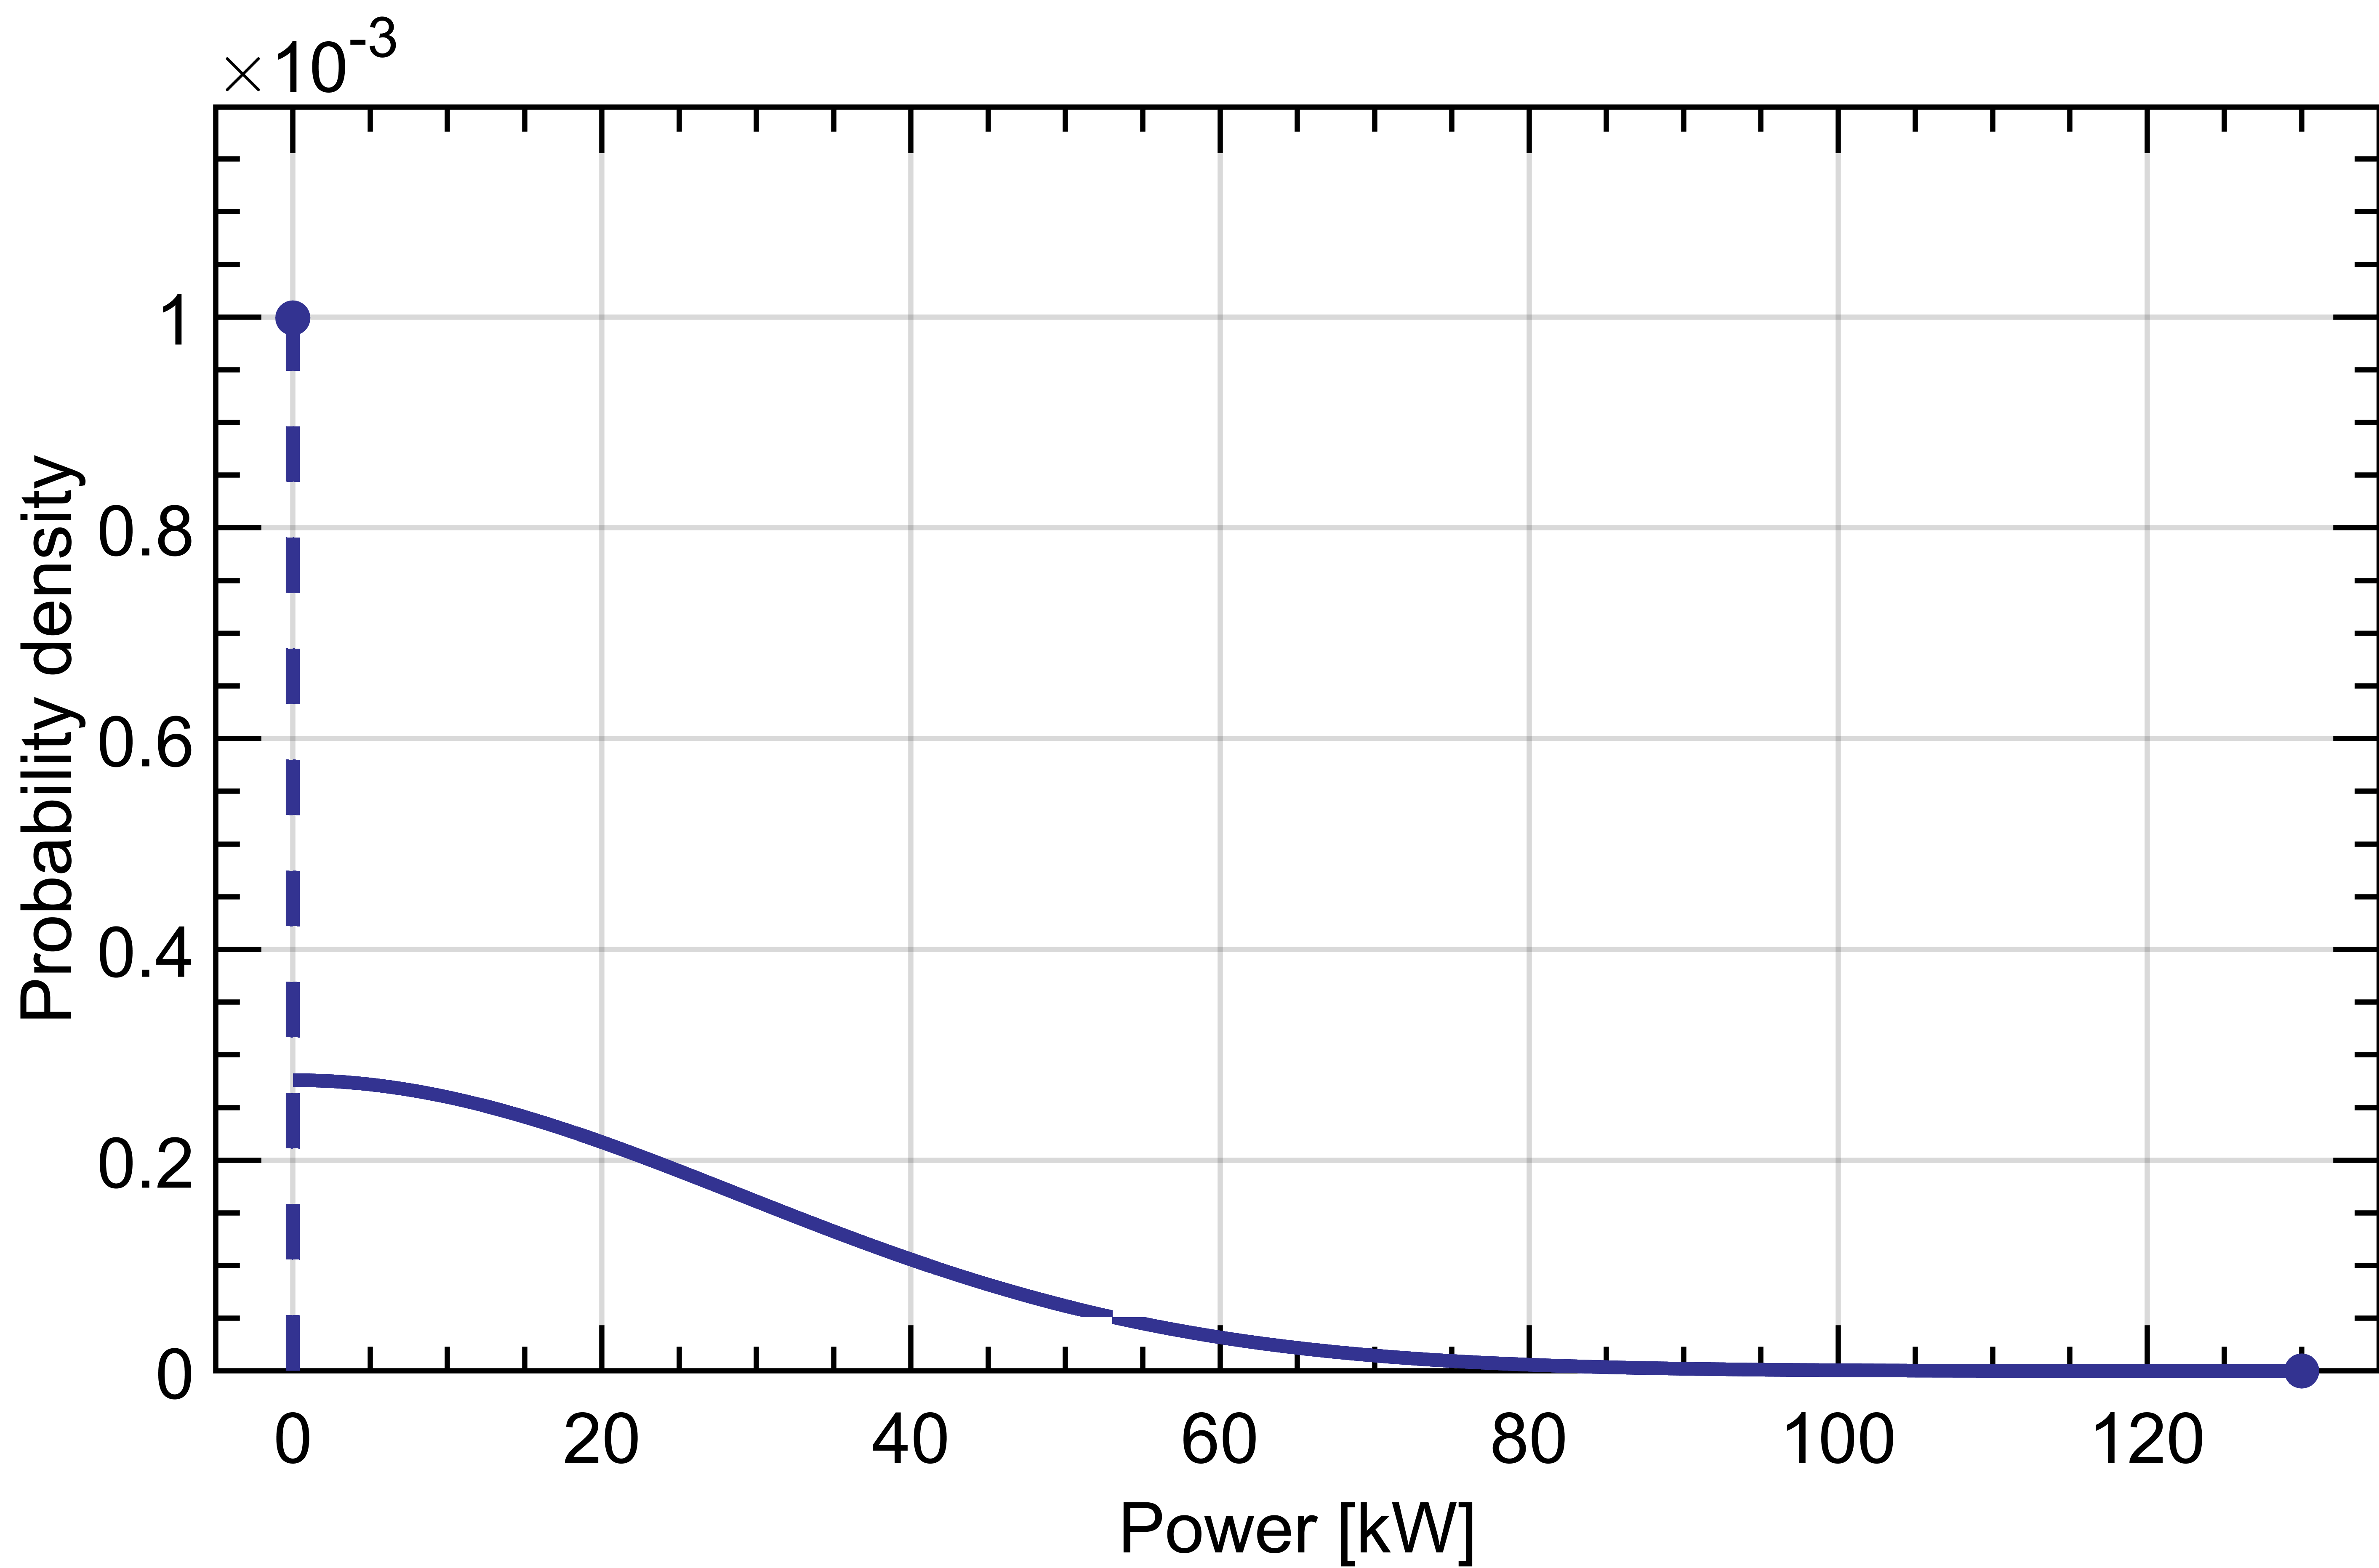
\includegraphics[width=0.4\textwidth]{02-figures/esempioFigura.png}
\caption{Esempio figura.}
\label{fig:Prova1}
\end{figure}

\begin{figure}[t!]
\centering
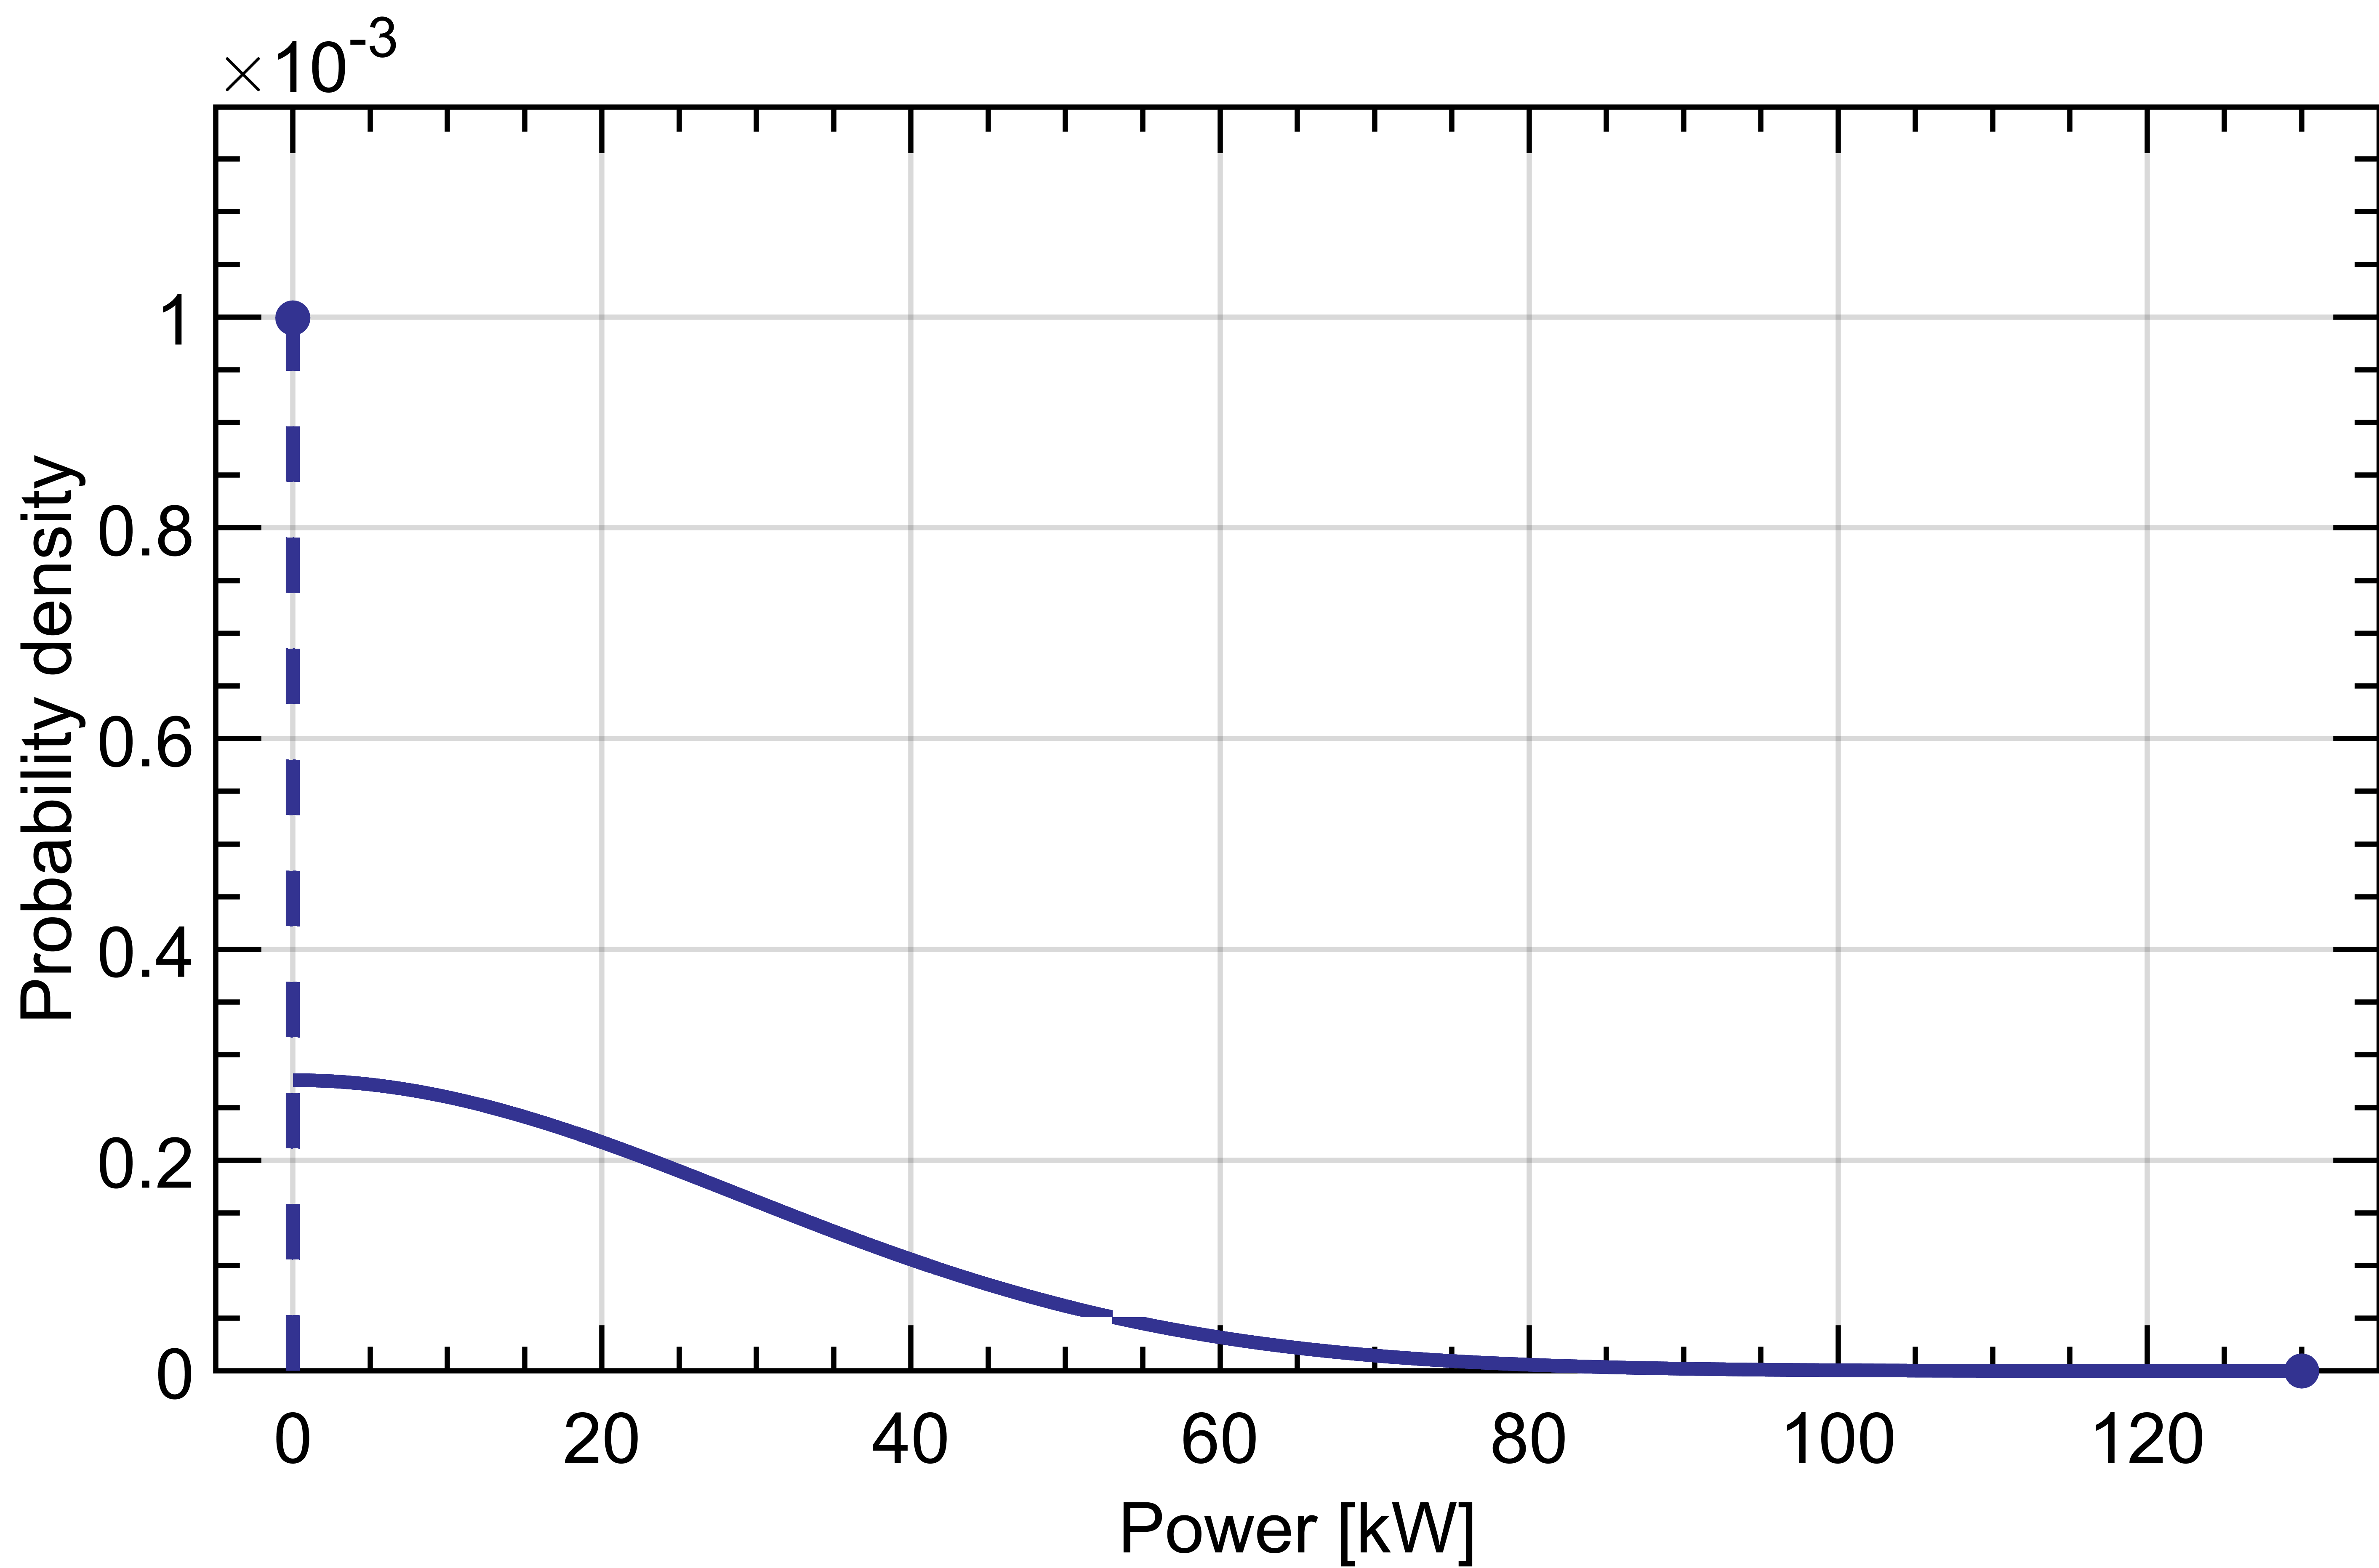
\includegraphics[width=1\textwidth]{02-figures/esempioFigura.png}
\caption{Esempio figura.}
\label{fig:Prova2}
\end{figure}

\newpage
\begin{figure}[H]
\centering
\subfloat[]{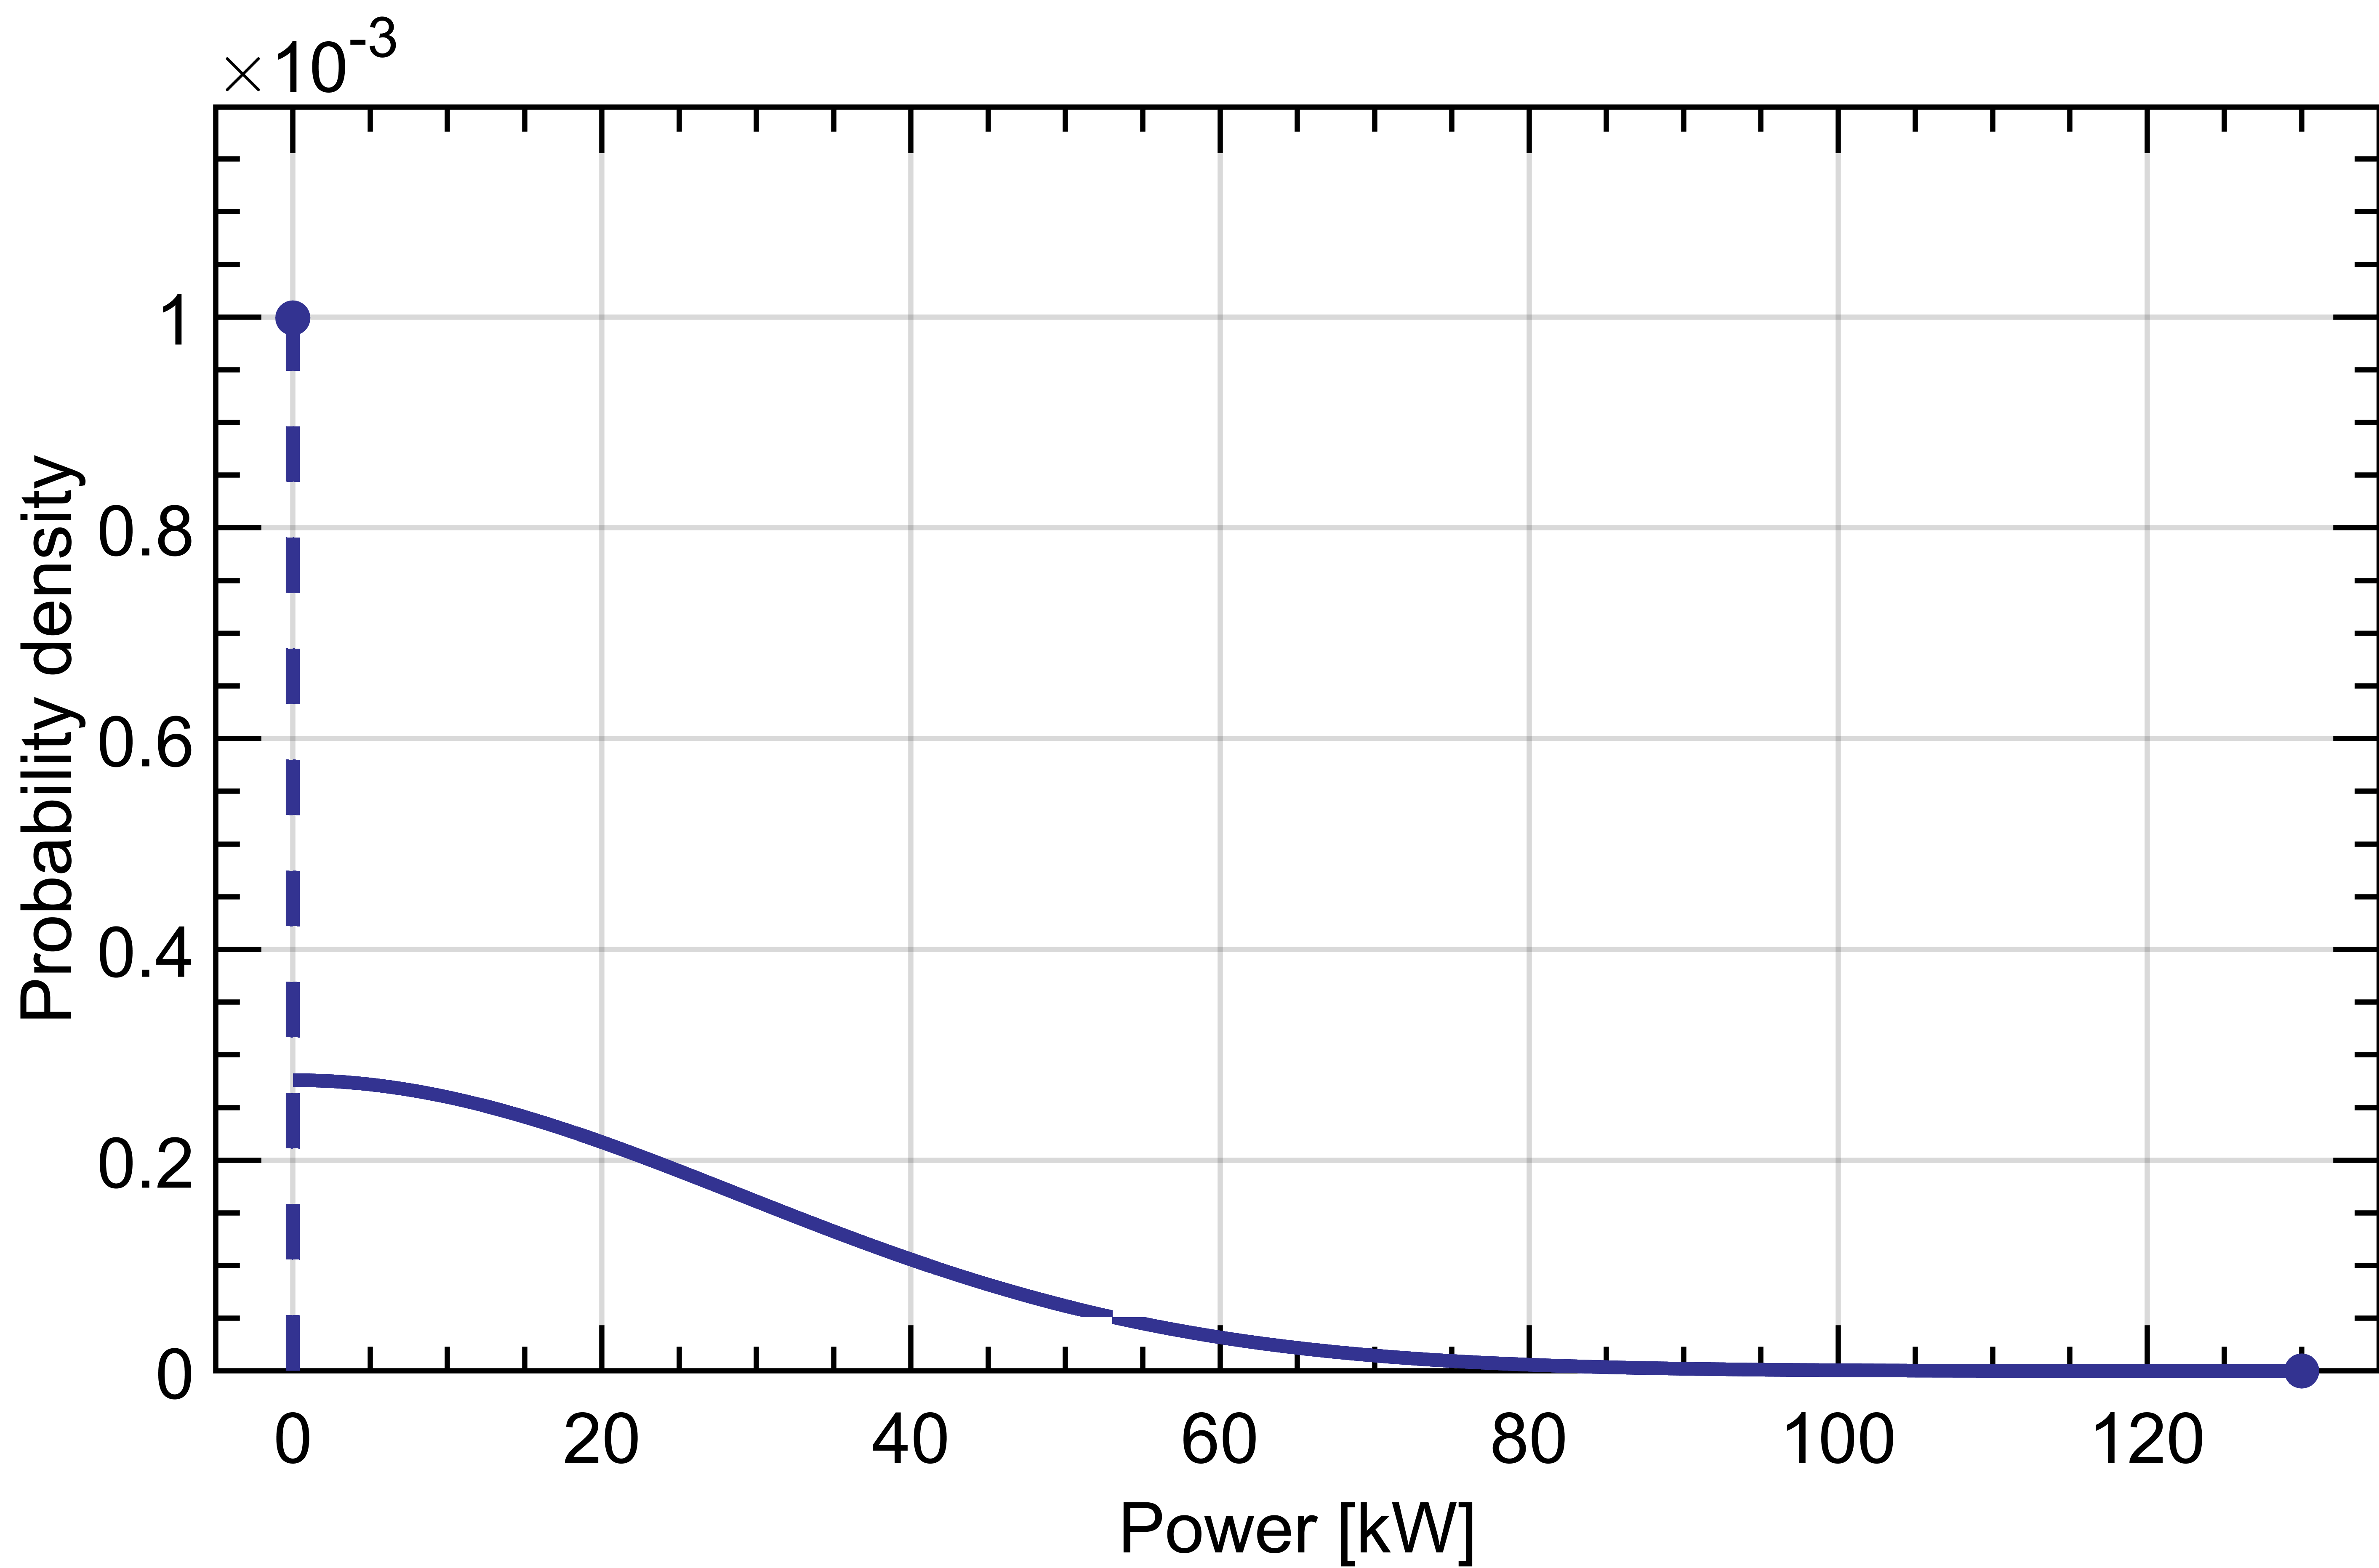
\includegraphics[width=0.45\textwidth]{02-figures/esempioFigura.png}}\hspace{0.1cm}
\subfloat[]{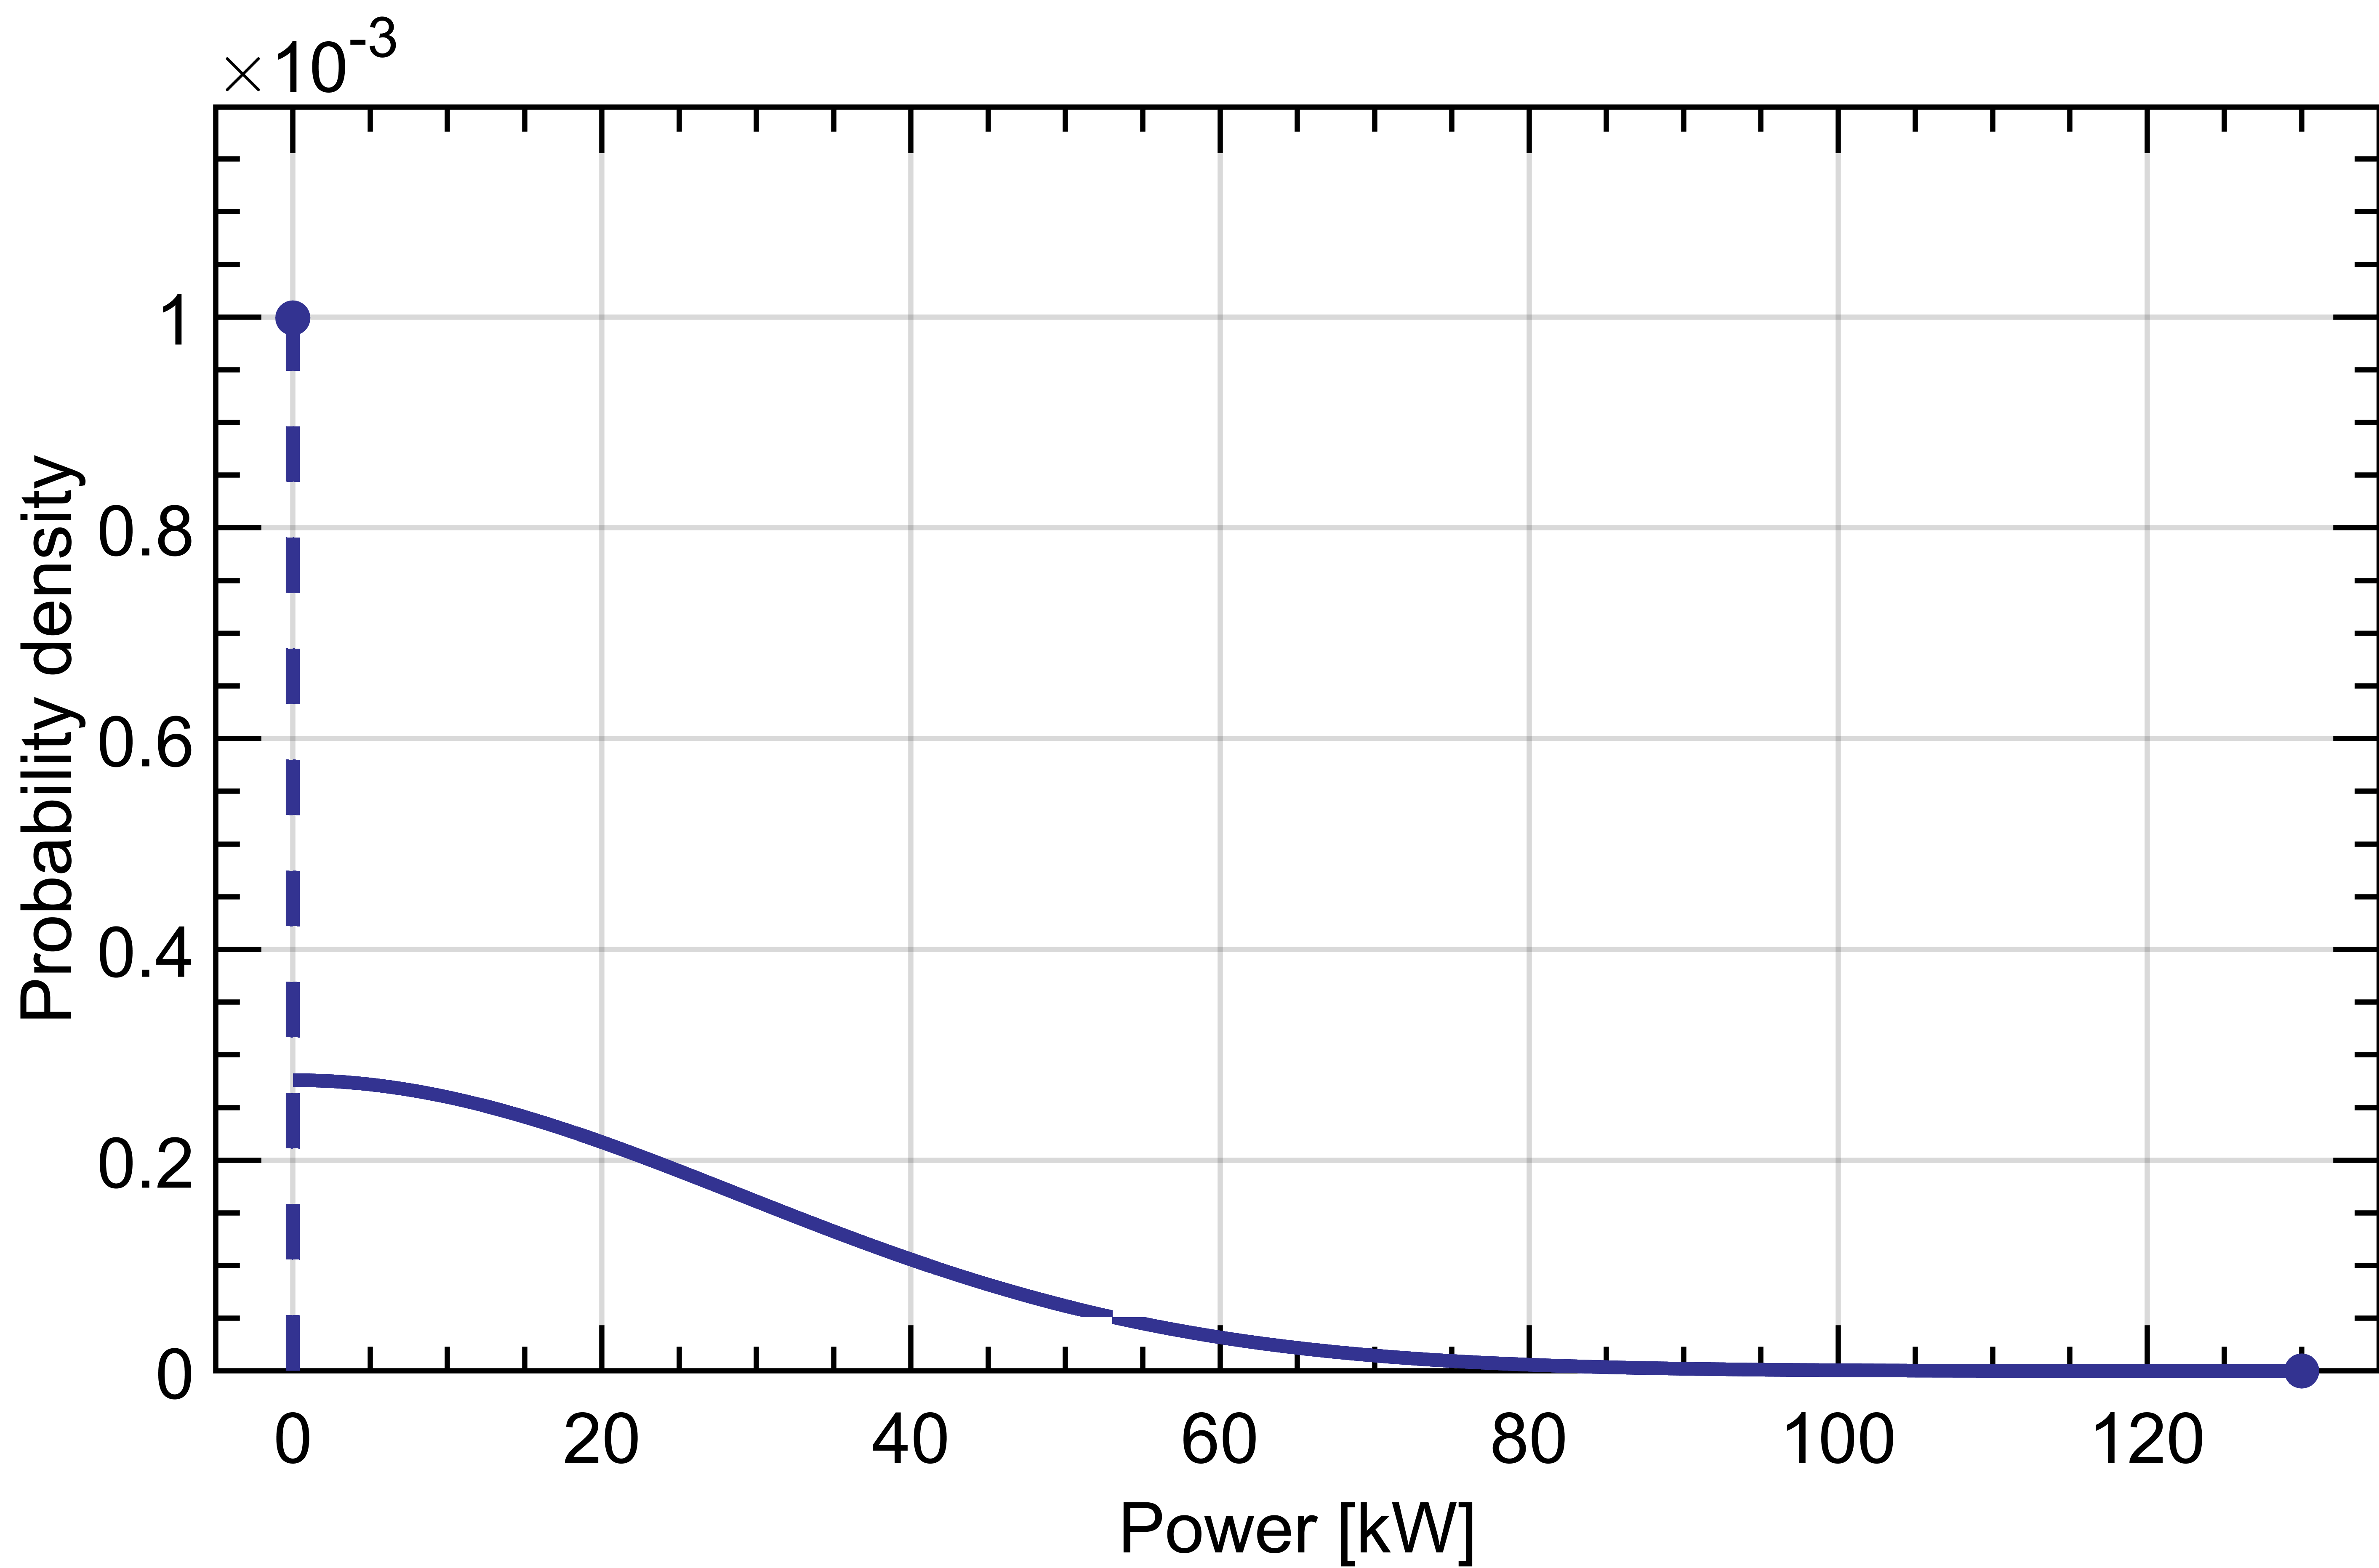
\includegraphics[width=0.45\textwidth]{02-figures/esempioFigura.png}}  \\
\caption{Esempio: (a) ..... e (b) .....}
\label{fig:5}
\end{figure}

Usare figure in .jpg o .png aumenta le dimensioni del file e ne riduce la qualità di stampa. Una soluzione può essere l'utilizzo di immagini in .pdf se sono schemi costruiti in Powerpoint oppure in .eps se figure generate in Matlab.
La figura \ref{fig:Prova1} è posizionata in alto, questo poiché è stato utilizzato il comando "t!". Per una panoramica sulle opzioni relative al posizionamento di figure, tabelle e algoritmi consultare \url{https://it.overleaf.com/learn/latex/Positioning_of_Figures}.

\begin{figure}[H]
\centering
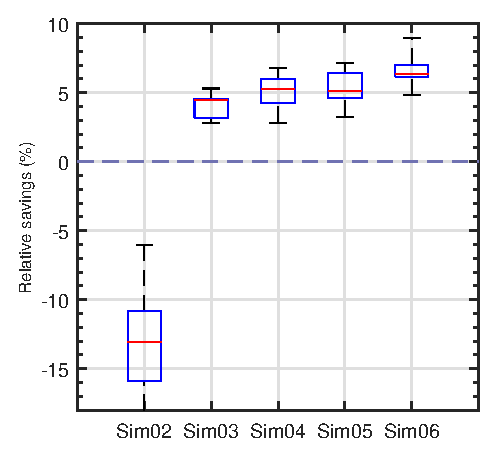
\includegraphics[width=0.6\textwidth]{02-figures/esempioFigura2.eps}
\caption{Esempio figura in formato eps.}
\label{fig:Prova3}
\end{figure}

\begin{figure}[H]
\centering
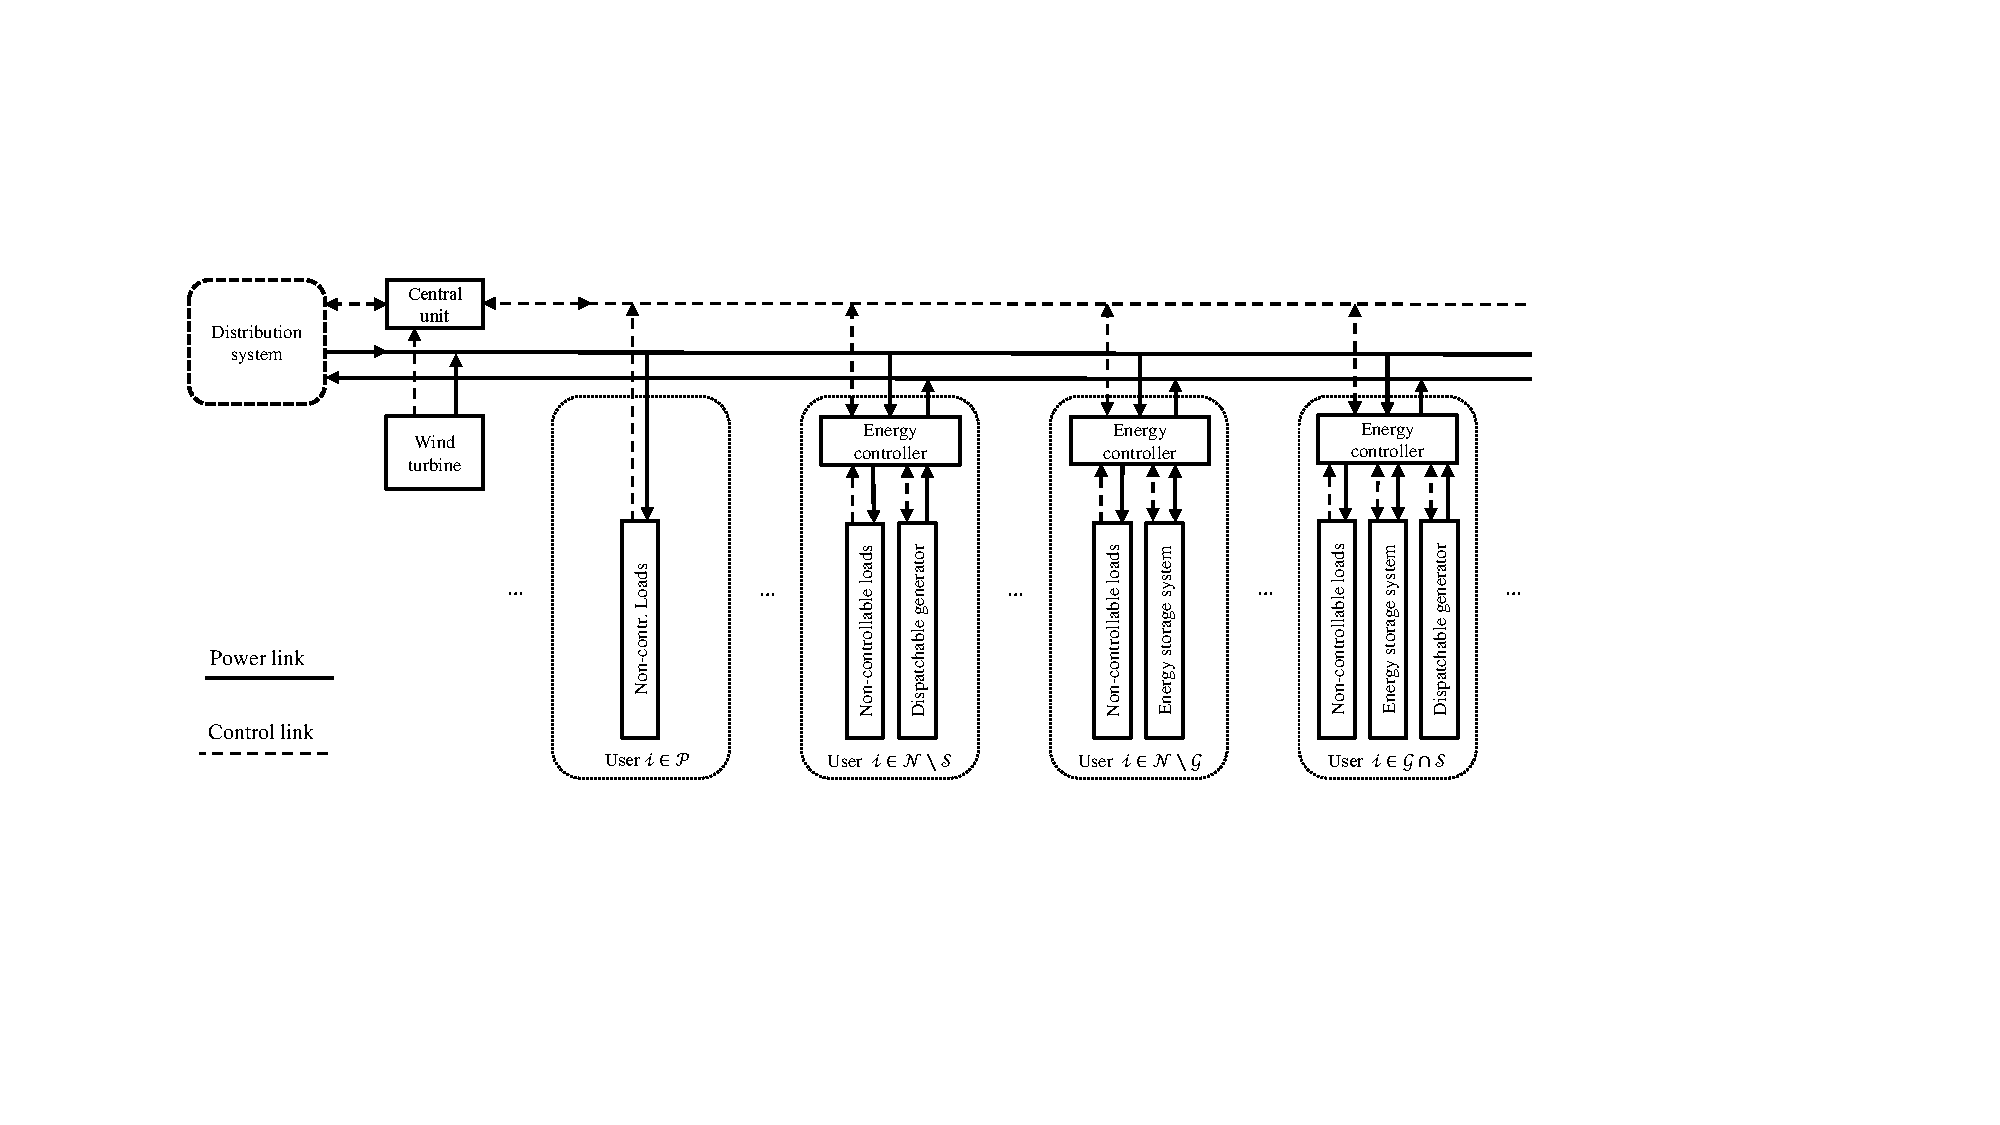
\includegraphics[width=\textwidth]{02-figures/esempioFigura3.pdf}
\caption{Esempio figura in pdf.}
\label{fig:Prova4}
\end{figure}

\subsection{Teoremi, definizioni, ecc.}
Il modello mette a disposizione gli ambienti "teorema", "definizione", "lemma" e "corollario", numerati automaticamente.
\begin{teorema}
Enunciato del teorema.
\end{teorema}

\begin{definizione}
Enunciato della definizione.
\end{definizione}

\begin{lemma}
Enunciato del lemma.
\end{lemma}

\begin{corollario}
Enunciato del corollario.
\end{corollario}


\begin{lstlisting}[language=Python]
    
\end{lstlisting}
\chapter{Stato dell'arte}
\label{capitolo2}

Nella seconda sezione si riporta lo stato dell'arte del settore, un inquadramento dell'area di ricerca orientato a portare il lettore all'interno della problematica affrontata. Bisogna dimostrare di conoscere le cose fatte fino ad ora in questo campo e il perché si sia reso necessario lo svolgimento di questo lavoro. Questa sezione deve essere grondante di citazioni bibliografiche.

\chapter{Impostazione del problema di ricerca}
\label{capitolo3}

In questa sezione si deve descrivere l'obiettivo della ricerca, le problematiche affrontate ed eventuali definizioni preliminari nel caso la tesi sia di carattere teorico.
\chapter{Architettura del sistema}
\label{capitolo4}

Si mostra il progetto dell'architettura del sistema con i vari moduli.

\chapter{Simulazioni numeriche}
\label{capitolo5}

Si mostra il progetto dal punto di vista sperimentale, le cose materialmente realizzate. In questa sezione si mostrano le attività sperimentali svolte, si illustra il funzionamento del sistema (a grandi linee) e si spiegano i risultati ottenuti con la loro valutazione critica. Bisogna introdurre dati sulla complessità degli algoritmi e valutare l'efficienza del sistema.
\chapter{Direzioni future di ricerca e conclusioni}
\label{capitolo6}

Si mostrano le prospettive future di ricerca nell'area dove si è svolto il lavoro. Talvolta questa sezione può essere l'ultima sottosezione della precedente. Nelle conclusioni si deve richiamare l'area, lo scopo della tesi, cosa è stato fatto,come si valuta quello che si è fatto e si enfatizzano le prospettive future per mostrare come andare avanti nell'area di studio.
%%%%%%%%%%%%%%%%%%%%%%%%%%%%%%%%%%%%%%%%%%%%%%%%%%%%%%%%%%%%%%

%% Bibliografia (non modificare)
\backmatter
\printbibliography[heading=bibintoc,title={Riferimenti}]
%\printbibliography[heading=bibintoc,title={References}] % Per tesi in inglese decommentare
%%%%%%%%%%%%%%%%%%%%%%%%%%%%%%%%%%%%%%%%%%%%%%%%%%%%%%%%%%%%%%

%% Appendice (aggiungere o rimuovere)
\appendix
\chapter{Codici}
\label{appendiceA}

I codici vanno caricati direttamente su Overleaf, nella sottocartella corrispondente al linguaggio (03-code/matlab oppure 03-code/python), e richiamati nel testo con "lstinputlisting".

\section{Matlab}
\lstinputlisting{03-code/matlab/Codice1.m}

\section{Python}
Per il codice Python si usa lo stile "pythonstyle" definito nel pacchetto del laboratorio:
\lstinputlisting[style=pythonstyle]{03-code/python/Codice1.py}
%%%%%%%%%%%%%%%%%%%%%%%%%%%%%%%%%%%%%%%%%%%%%%%%%%%%%%%%%%%%%%
\end{document}